\documentclass[a4paper,10pt,oneside]{book}
\usepackage[utf8]{inputenc}
\usepackage{parskip}
\usepackage{graphicx}
\usepackage{caption}
\usepackage{multirow}
\usepackage{wrapfig}
\usepackage{array}
\usepackage{longtable}
\usepackage[hidelinks]{hyperref}
\usepackage[margin=2.5cm]{geometry}

\title{Notes on Navigation}
\author{Philip Bradley}
\date{March 2019}

\begin{document}
\raggedbottom

\maketitle
\tableofcontents

\chapter{Shapes, Lights and Sounds}

For vessels at sea, the rules of the road are defined by the
International Regulations for the Prevention of Collisions at Sea (IRPCS
or COLREGS), a set of rules published by International Maritime
Organisation (IMO) in 1972.

The COLREGS include a set of audio and visual signals that allow vessels
to identify each other during the day (days shapes), at night (lights)
and in restricted visibility/fog (sound signals).


\section{Day Shapes}

These are black geometric shapes, hung from a mast, to indicate the operational status of a vessel. The shapes used are designed to be recognisable from any viewing angle (ball, cylinder, cone, diamond).

\begin{center}
   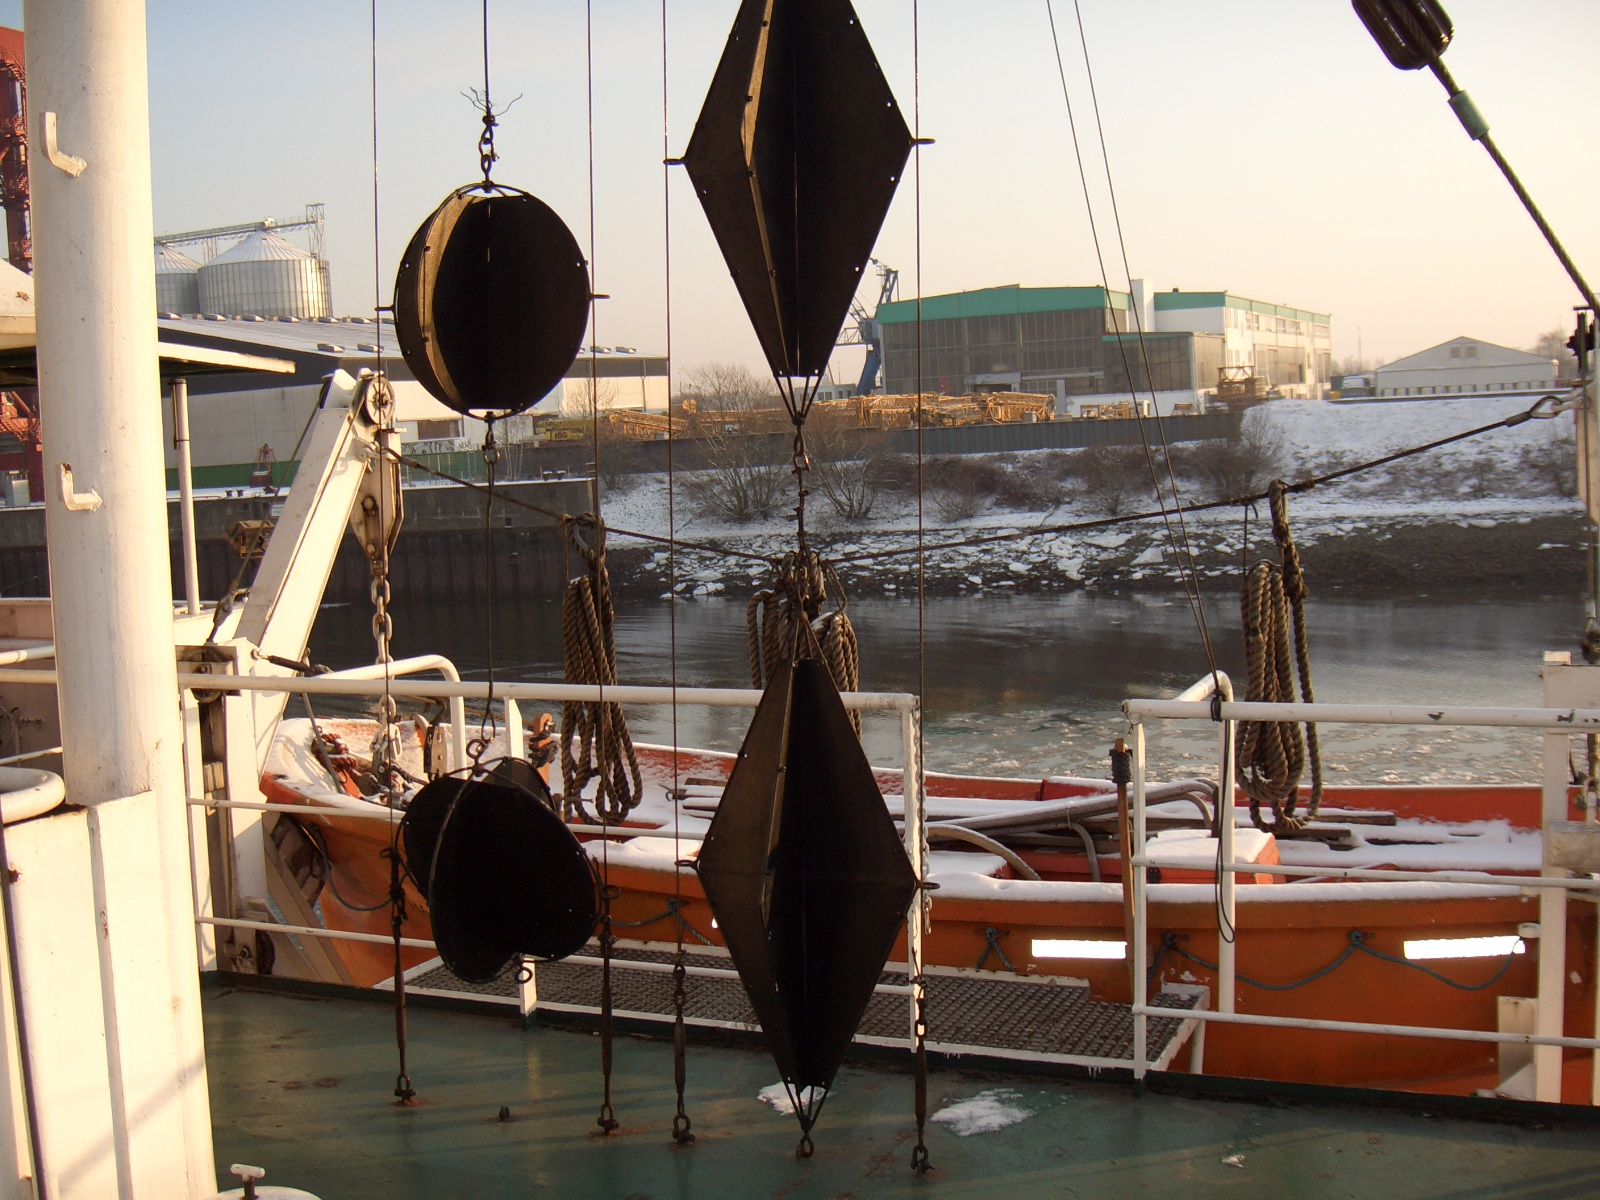
\includegraphics[width=0.9\linewidth,keepaspectratio=true]
   {resources/Day_Shapes.png}
   \captionof{figure}{Day Shapes}
   \vspace{20pt}
\end{center}

\newpage
The following are some commonly used shapes:

\renewcommand{\arraystretch}{1.5}
\begin{tabular}{|c|>{\centering\arraybackslash}m{0.4\linewidth}|}
\hline
Power underway & No shape required \\

\hline
Yacht sailing  & No shape required \\

\hline
Tug Towing & 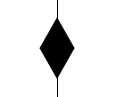
\includegraphics[width=0.3\linewidth]{resources/Shape_Diamond.png} \\

\hline
Fishing & 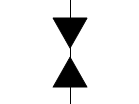
\includegraphics[width=0.3\linewidth]{resources/Shape_2Cone.png} \\

\hline
Trawling  & 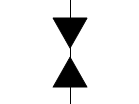
\includegraphics[width=0.3\linewidth]{resources/Shape_2Cone.png} \\

\hline
Limited by draught  & 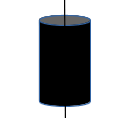
\includegraphics[width=0.3\linewidth]{resources/Shape_Cylender.png} \\

\hline
Restricted ability to manoeuvre & 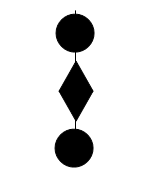
\includegraphics[width=0.3\linewidth]{resources/Shape_RAM.png} \\

\hline
Not under command & 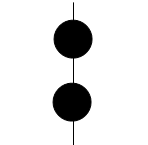
\includegraphics[width=0.3\linewidth]{resources/Shape_2Ball.png} \\

\hline
Anchored & 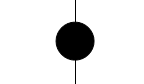
\includegraphics[width=0.3\linewidth]{resources/Shape_Ball.png} \\

\hline
Stopped & No shape required \\

\hline
Yacht motor sailing & 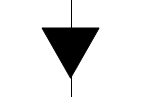
\includegraphics[width=0.3\linewidth]{resources/Shape_Cone.png} \\

\hline
Aground & 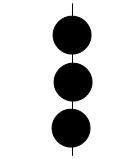
\includegraphics[width=0.3\linewidth]{resources/Shape_3Ball.png} \\

\hline
Dredging & 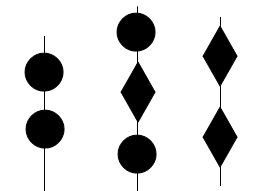
\includegraphics[width=0.3\linewidth]{resources/Shape_Dredge.png} \\
\hline

\end{tabular}

\newpage
Also of note is that a diving vessel will display the international code flag A as shown below:

\begin{center}
   
\includegraphics[width=0.3\linewidth,keepaspectratio=true]
   {resources/Flag_A.png}
   \captionof{figure}{Flag A}
   \vspace{20pt}
\end{center}


\section{Sound Signals for Vessels in Restricted Visibility}

The following sound signals should be emitted by vessels in restricted visibility conditions every 2 minutes. The short blast should be about 1 second in duration while long blasts should be 4 – 6 seconds.


\begin{center}
  \begin{tabular}{|c|c|}
  \hline
  Power Underway &   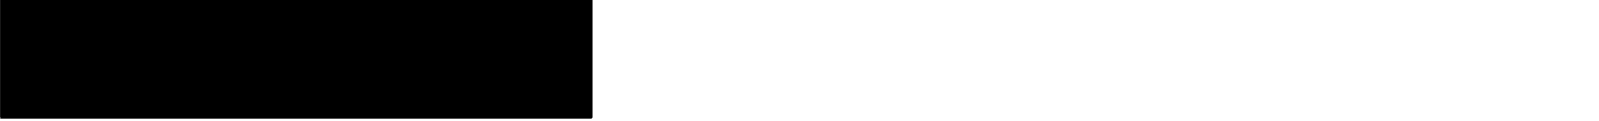
\includegraphics[width=0.2\linewidth]{resources/Sounds/Sound-long.png}
  \\
  \hline
  Yacht sailing & 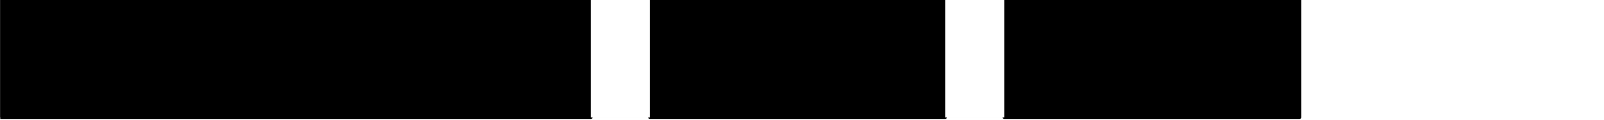
\includegraphics[width=0.2\linewidth]{resources/Sounds/Sound-long-short-short.png}\\
  \hline
  Tug Towing & 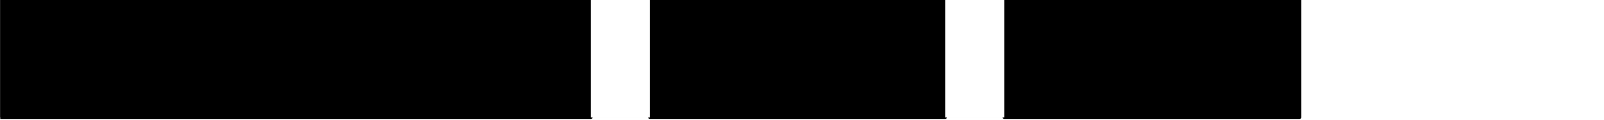
\includegraphics[width=0.2\linewidth]{resources/Sounds/Sound-long-short-short.png}\\
  \hline
  Fishing & 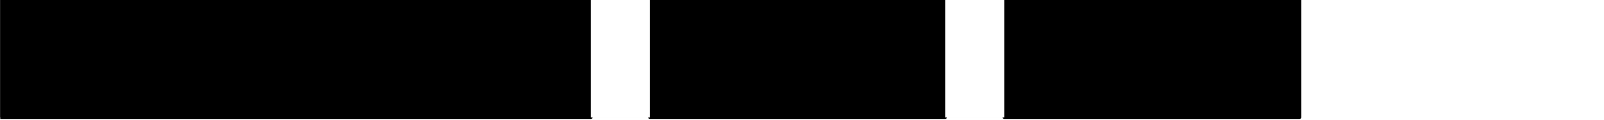
\includegraphics[width=0.2\linewidth]{resources/Sounds/Sound-long-short-short.png}\\
  \hline
  Trawling & 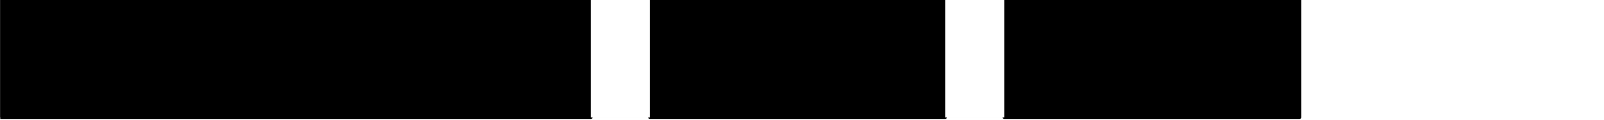
\includegraphics[width=0.2\linewidth]{resources/Sounds/Sound-long-short-short.png}\\
  \hline
  Limited by draught & 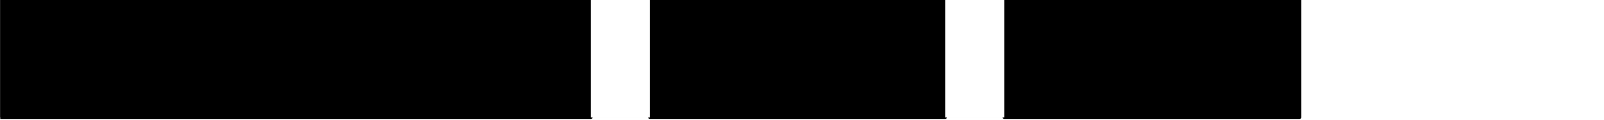
\includegraphics[width=0.2\linewidth]{resources/Sounds/Sound-long-short-short.png}\\
  \hline
  Limited by manoeuvre & 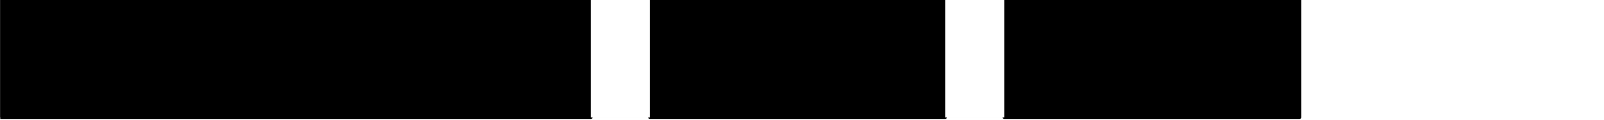
\includegraphics[width=0.2\linewidth]{resources/Sounds/Sound-long-short-short.png}\\
  \hline
  Not under command & 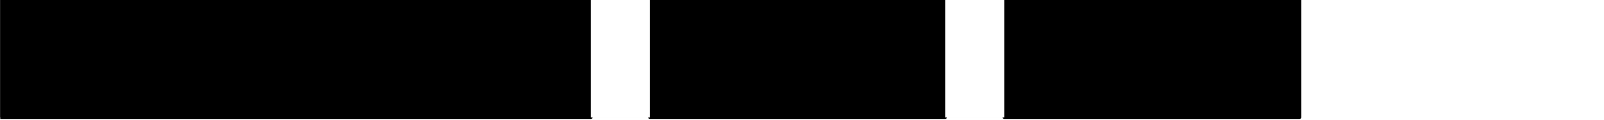
\includegraphics[width=0.2\linewidth]{resources/Sounds/Sound-long-short-short.png}\\
  \hline
  Anchored & 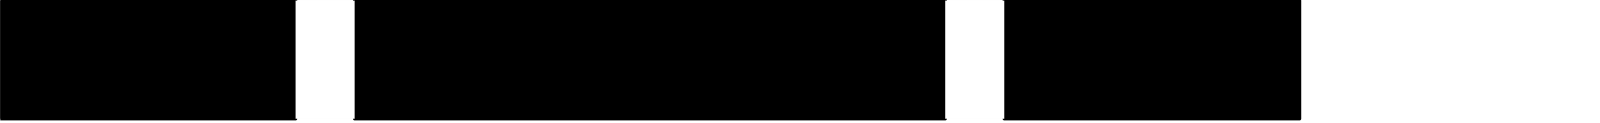
\includegraphics[width=0.2\linewidth]{resources/Sounds/Sound-short-long-short.png}\\
  \hline
  Stopped & 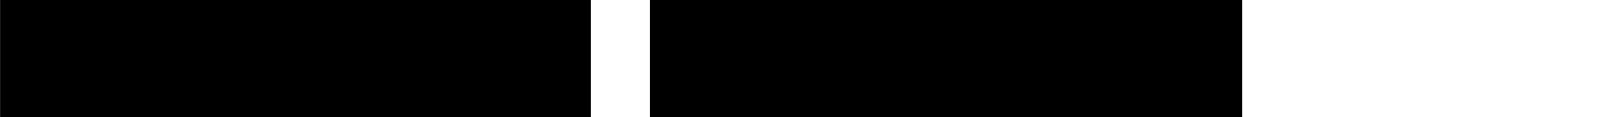
\includegraphics[width=0.2\linewidth]{resources/Sounds/Sound-long-long.png}\\
  \hline
  Yacht motor sailing & 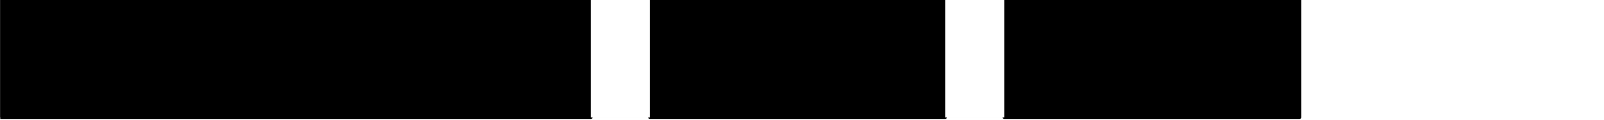
\includegraphics[width=0.2\linewidth]{resources/Sounds/Sound-long-short-short.png}\\
  \hline
  Vessel being towed (if manned) & 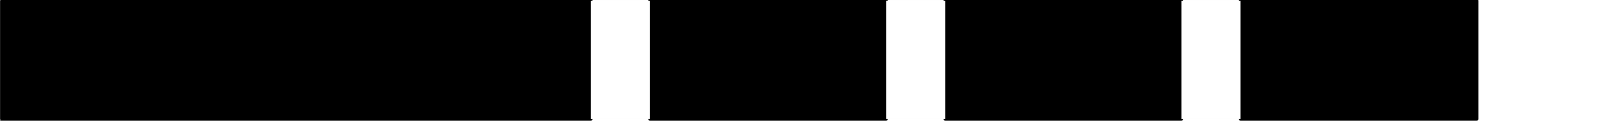
\includegraphics[width=0.2\linewidth]{resources/Sounds/Sound-long-short-short-short.png}\\
  \hline
  \end{tabular}
\end{center}

\newpage
\vspace{20pt}
Additional lights on the mast are used to indicate the operational status of the vessel. Some of these are listed below:

\begin{longtable}{|c|c|}
\hline
Power Underway &   No mast lights, just navigation and stern white light \\
\hline
Yacht sailing & No mast lights, just navigation and stern white light \\
\hline
Tug Towing & 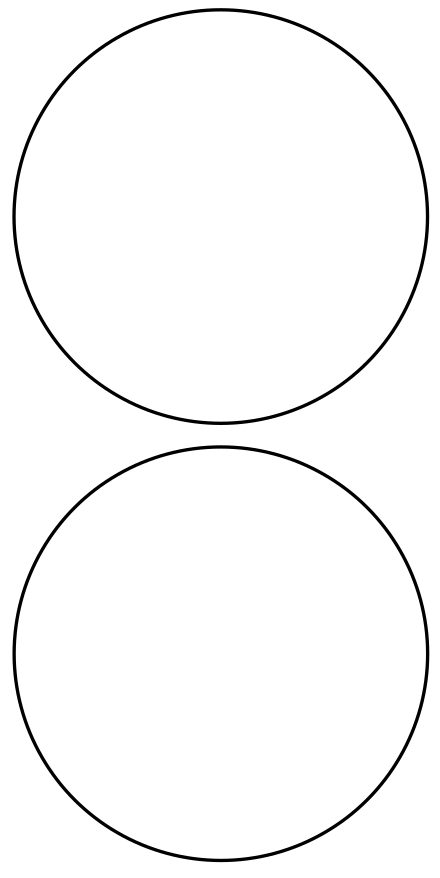
\includegraphics[width=0.1\linewidth]{resources/Nav_lights/Lights-white-white.png}\\
\hline
Fishing & 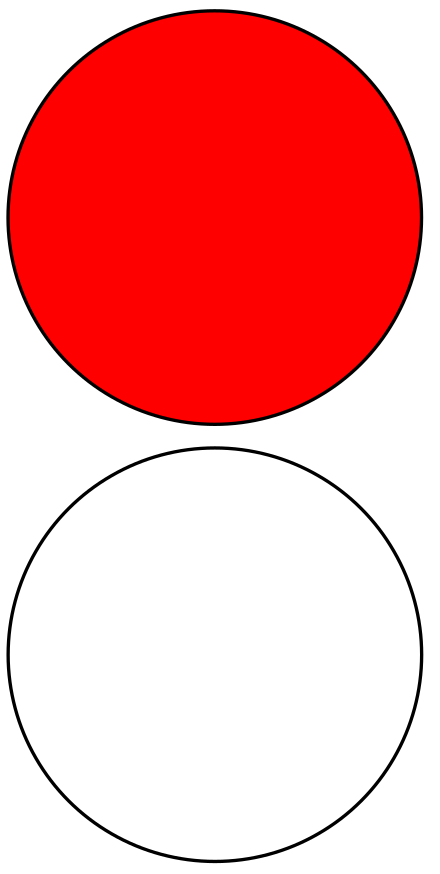
\includegraphics[width=0.1\linewidth]{resources/Nav_lights/Lights-red-white.png}\\
\hline
Trawling & 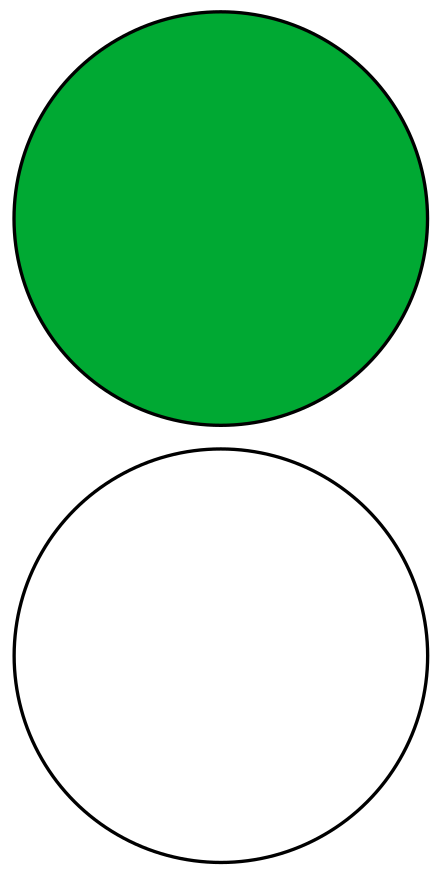
\includegraphics[width=0.1\linewidth]{resources/Nav_lights/Lights-green-white.png}\\
\hline
Limited by draught & 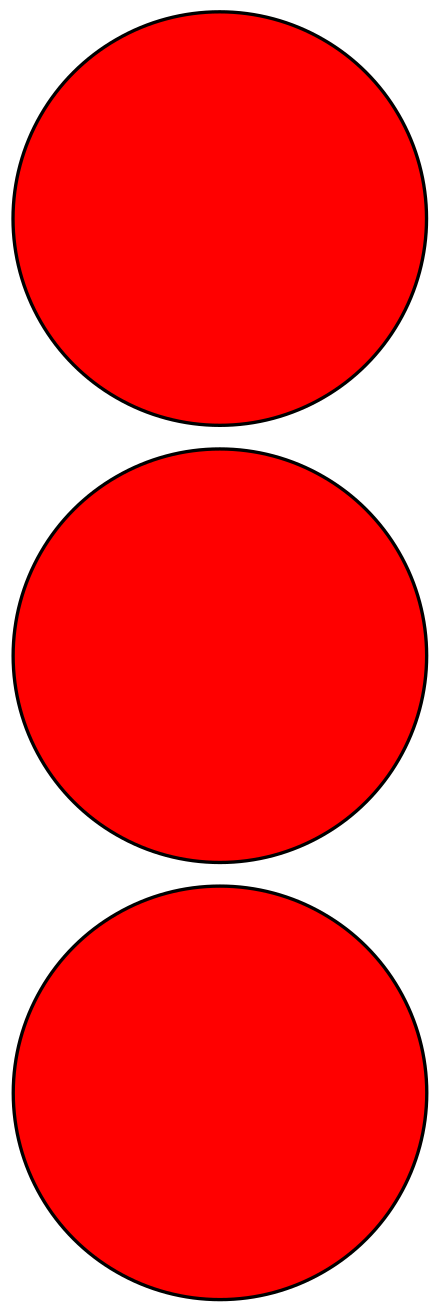
\includegraphics[width=0.1\linewidth]{resources/Nav_lights/Lights-red-red-red.png}\\
\hline
Limited by manoeuvre & 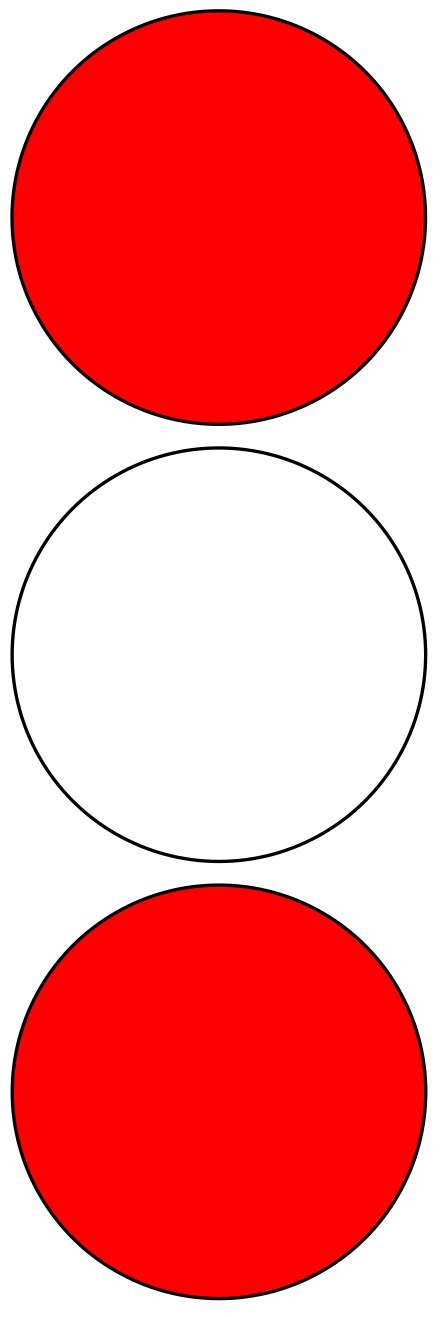
\includegraphics[width=0.1\linewidth]{resources/Nav_lights/Lights-red-white-red.png}\\
\hline
Not under command & 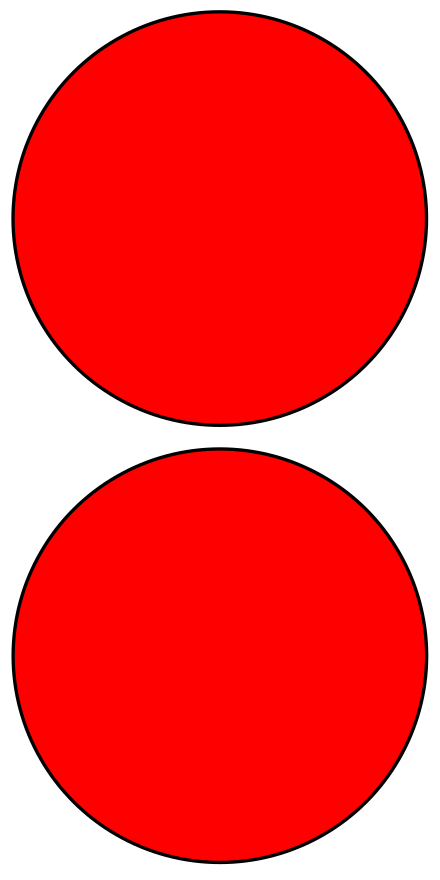
\includegraphics[width=0.1\linewidth]{resources/Nav_lights/Lights-red-red.png}\\
\hline
Anchored & 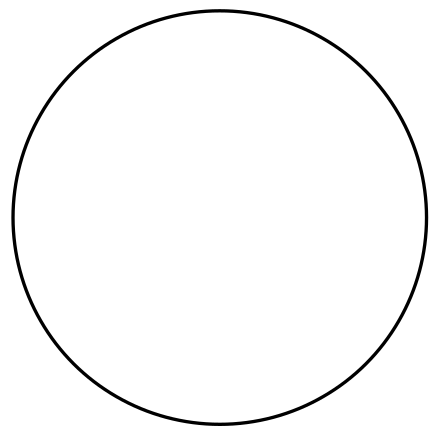
\includegraphics[width=0.1\linewidth]{resources/Nav_lights/Lights-white.png}\\
\hline
Stopped & 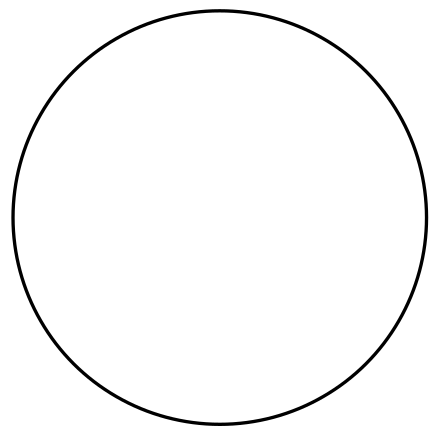
\includegraphics[width=0.1\linewidth]{resources/Nav_lights/Lights-white.png}\\
\hline
Yacht motor sailing & No mast lights, just navigation and  all round white light \\
\hline
\end{longtable}



\newpage
\section{Navigation Lights}
All vessels must display navigation lights between sunset and sunrise and also during times of restricted visibility.

All types of vessel should be equipped with side lights. The red light is always on the port/left side while the green is always on the starboard/right side.

A sailing vessel should display the sidelights along with a white light visible only from the stern. A power vessel should the sidelights along with a white masthead light visible from all directions. Vessels of more than 50m in length must display a second white masthead light. Note that a power vessel in this context could be a motor yacht.

\vspace{20pt}

\begin{center}
\begin{minipage}{0.45\linewidth}
  \centering
  
\includegraphics[width=0.8\linewidth]{resources/Nav_Lights_Sailing.png}
  \captionof{figure}{Sailing vessel, white light is only visible from the stern}
\end{minipage}
\hfill
\begin{minipage}{0.45\linewidth}
  \centering
  
\includegraphics[width=0.8\linewidth]{resources/Nav_Lights_Motor.png}
  \captionof{figure}{Power vessel, white light is visible from all aspects}
\end{minipage}
\end{center}
\vspace{20pt}


Additional lights on the mast are used to indicate the operational status of the vessel. Some of these are listed below:


\newpage
\subsection{Example Silhouettes}

\begin{longtable}{|c|c|}
	\hline
	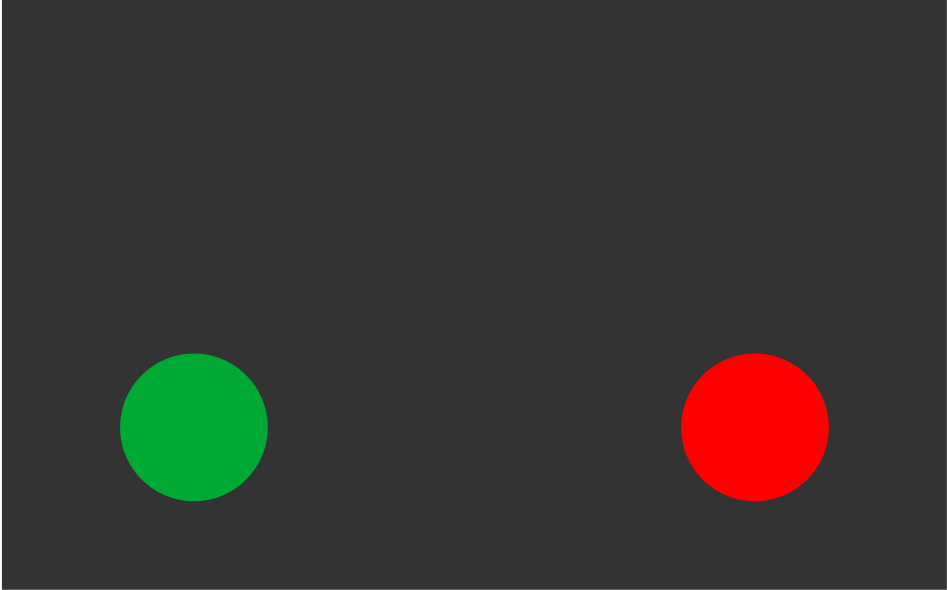
\includegraphics[width=0.3\linewidth]{resources/Nav_lights/Sil-green-red.png} & Sailing vessel underway, viewed bow-on (heading towards the viewer) \\
	\hline
	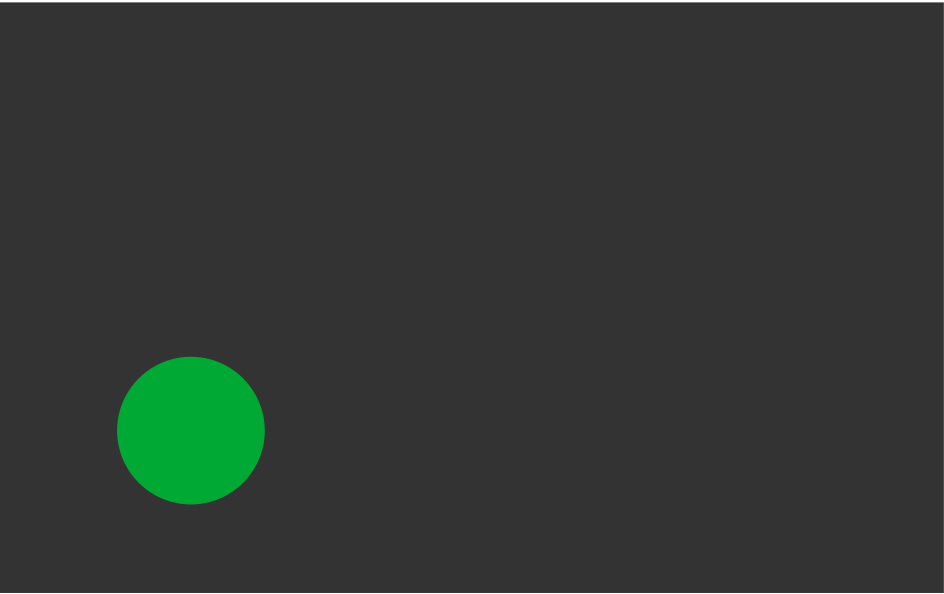
\includegraphics[width=0.3\linewidth]{resources/Nav_lights/Sil-green.png} & Sailing vessel underway, viewed from starboard side \\
	\hline
	
\includegraphics[width=0.3\linewidth]{resources/Nav_lights/Sil-red.png} & Sailing vessel underway, viewed from port side \\
	\hline
	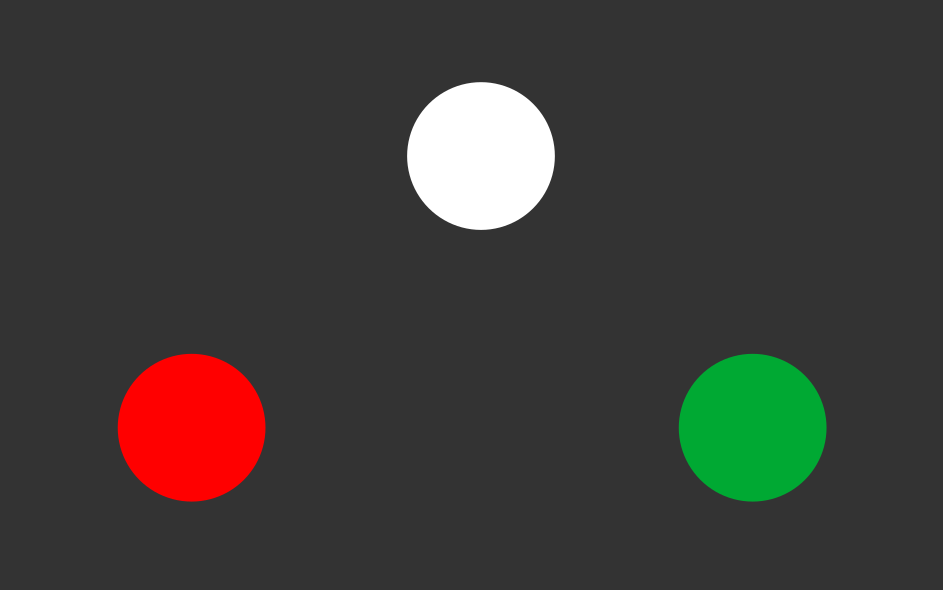
\includegraphics[width=0.3\linewidth]{resources/Nav_lights/Sil-red-white-green.png} & Sailing vessel viewed from the stern or Motor vessel viewed from the stern \\	
	\hline	
	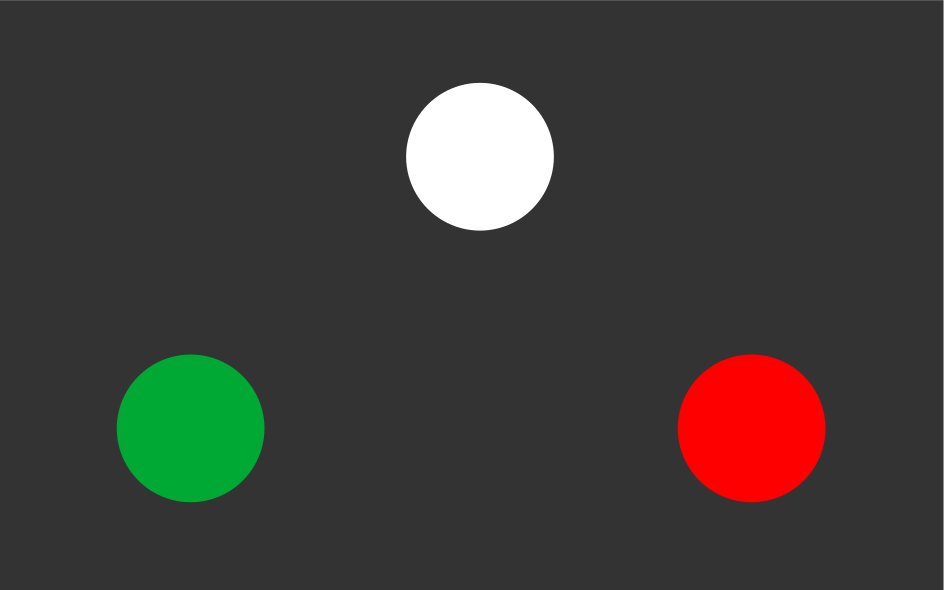
\includegraphics[width=0.3\linewidth]{resources/Nav_lights/Sil-green-white-red.png} & Motor vessel viewed bow-on \\	
	\hline	
	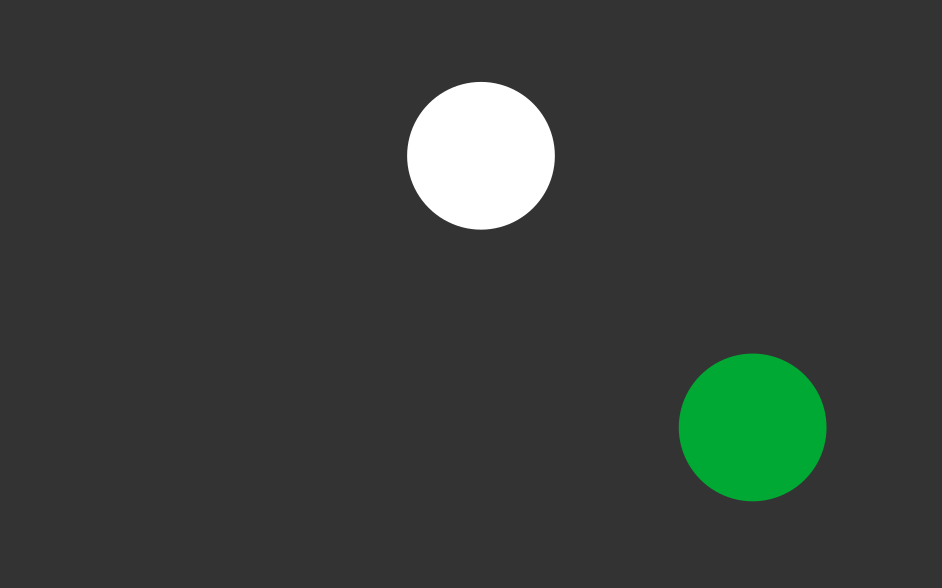
\includegraphics[width=0.3\linewidth]{resources/Nav_lights/Sil-white-green.png} & Motor vessel underway, viewed from starboard side\\	
	\hline	
	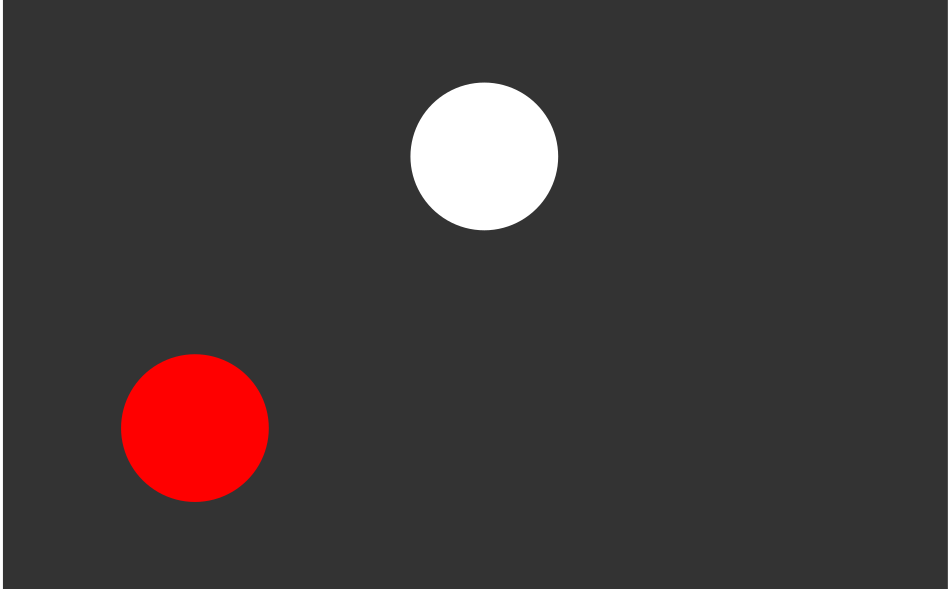
\includegraphics[width=0.3\linewidth]{resources/Nav_lights/Sil-red-white.png} & Motor vessel underway, viewed from the port side\\	
	\hline		
	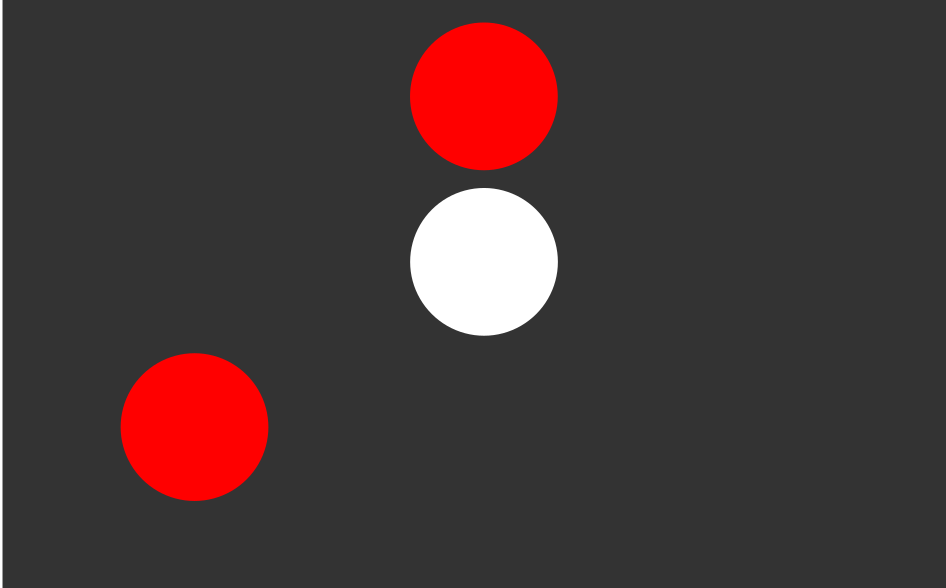
\includegraphics[width=0.3\linewidth]{resources/Nav_lights/Sil-red-red-white.png} & Fishing vessel, viewed from the port side \\	
	\hline		
	
\includegraphics[width=0.3\linewidth]{resources/Nav_lights/Sil-white.png} & Anchored \emph{or} Stopped \emph{or} Sailing vessel viewed from stern \\	
	\hline		
	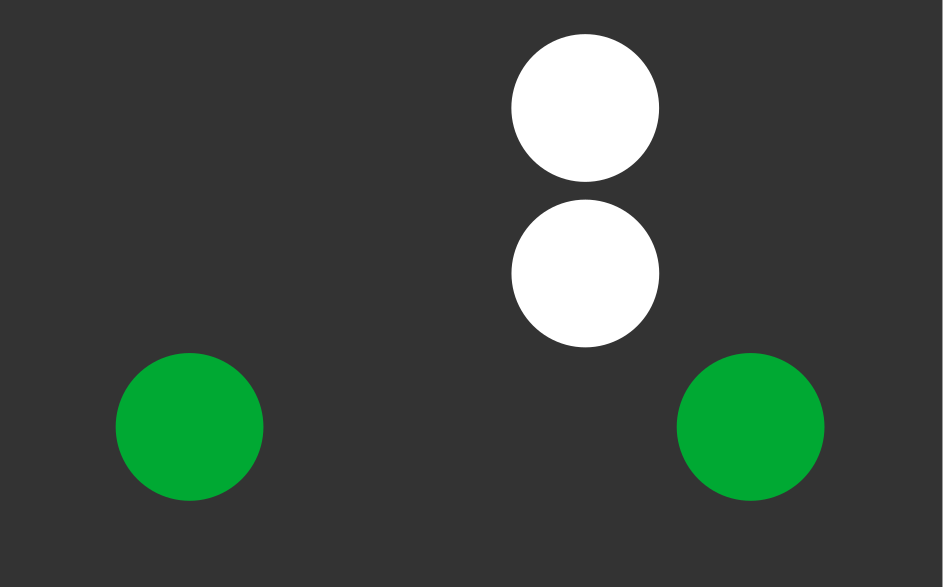
\includegraphics[width=0.3\linewidth]{resources/Nav_lights/Sil-green-white-white-green.png} & Towing vessel and vessel under tow, viewed from starboard side \\	
	\hline					
\end{longtable}	
	

\chapter{Bouyage Marks}
The International Association of Lighthouse Authorities (IALA) is an international organisation whose responsibilities include defining the Maritime Bouyage System (MBS) which includes:

\vspace{5pt}
\begin{itemize}
     \item Cardinal Marks
     \item Lateral Marks
     \item Special Marks
     \item Safe Water Marks
     \item Isolated Danger Marks
     \item New Danger Marks
\end{itemize}
\vspace{5pt}

While the IALA system is used worldwide, the meaning of red vs. green lateral marks depends on whether you are in Region B (Americas, Philippines, Japan and Korea) or Region A (the rest of the world). Only region A conventions are used in this document.


\newpage
\section{Cardinal Marks}
A cardinal mark is used to indicate the position the direction of safe water around a hazard. Cardinal marks indicate the direction of safety as a cardinal (compass) direction as opposed to lateral marks which indicate port and starboard relative to the direction of bouyage.

\begin{center}
   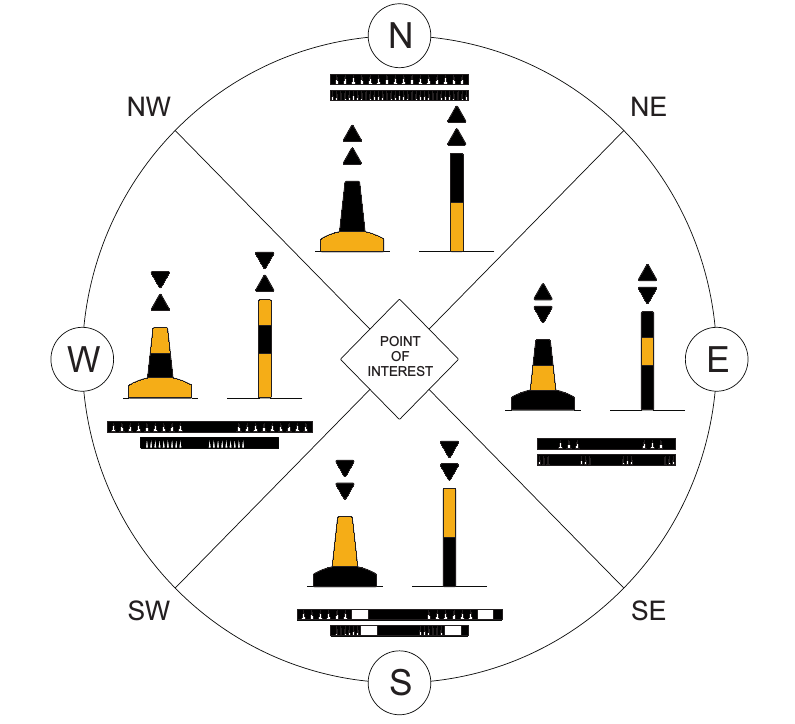
\includegraphics[width=0.9\linewidth,keepaspectratio=true]
   {resources/Cardinal_Marks.png}
   \captionof{figure}{Cardinal Marks}
   \vspace{20pt}
\end{center}



The diagram above shows all of the characteristics of the cardinal marks. As indicated, they can be either pillars or spars. Each mark is distinguished by:

\begin{itemize}
     \item The topmark (the arrows on top)
     \item The colour
     \item The light pattern (if fitted)
\end{itemize}


\newpage
\section{Lateral Marks}
A lateral mark is used to indicate the edge of the safe water channel. In Region A, for a vessel entering a harbour, the port side will indicated with red markers while the starboard side will be indicated with green markers.

While it might be obvious in many cases what is meant by “entering the harbour”, to avoid confusion, charts showing lateral marks must also indicate the “direction of bouyage” as shown in the schematic below:


\begin{center}
   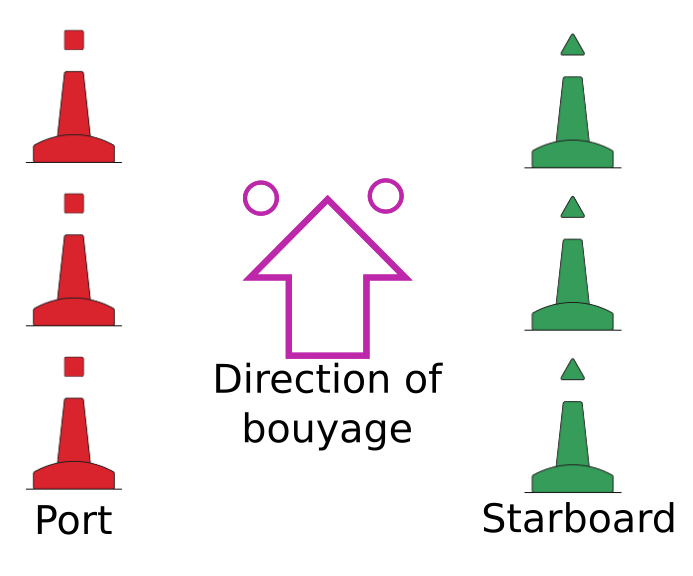
\includegraphics[width=0.9\linewidth,keepaspectratio=true]
   {resources/Lateral_Marks.png}
   \captionof{figure}{Lateral Marks}
   \vspace{20pt}
\end{center}

A more complete definition of the “direction of bouyage” is :

\begin{itemize}
 \item The general direction taken by the mariner when approaching a harbour, river, estuary or other waterway from seaward or
 \item The direction determined by the proper authority in consultation, where appropriate, with neighbouring countries.
\end{itemize}

Lateral marks come in different shapes, not just the “spar” shapes shown above. Port hand marks can be cylinders, spars or pillars:

\begin{center}
   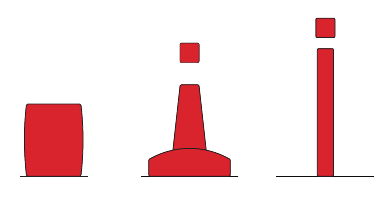
\includegraphics[width=0.9\linewidth,keepaspectratio=true]
   {resources/Laterals_Port.png}
   \captionof{figure}{Port Marks}
   \vspace{20pt}
\end{center}

while starboard hand marks can be cones, spars or pillars:

\begin{center}
   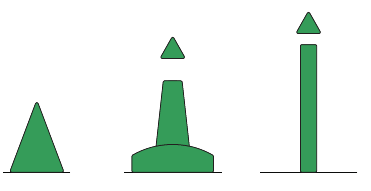
\includegraphics[width=0.9\linewidth,keepaspectratio=true]
   {resources/Laterals_Starboard.png}
   \captionof{figure}{Starboard Marks}
   \vspace{20pt}
\end{center}



\newpage
\section{Preferred Channel Indicators}
Where a channel splits, the preferred channel is indicated by modified lateral marks. Where the preferred channel is to port, the starboard mark will be modified to include a red stripe as below

\begin{center}
   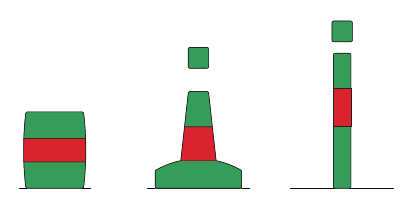
\includegraphics[width=0.9\linewidth,keepaspectratio=true]
   {resources/Channel_Starboard.png}
   \captionof{figure}{The starboard channel mark has been modified to indicate that the channel to the port is the preferred channel}
   \vspace{20pt}
\end{center}

Where the preferred channel is to starboard, the port channel mark will be modified to include a green stripe as below

\begin{center}
   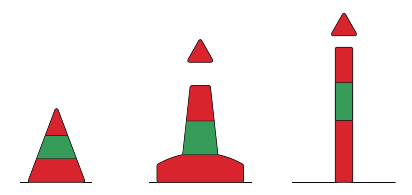
\includegraphics[width=0.9\linewidth,keepaspectratio=true]
   {resources/Channel_Port.png}
   \captionof{figure}{The port channel mark has been modified to indicate that the channel to the starboard is the preferred channel}
   \vspace{20pt}
\end{center}


In the example below, the preferred channel is on the port side. The starboard channel markers on the preferred channel have been modified to indicate this. The channel markers on the secondary channel are unchanged.

\begin{center}
   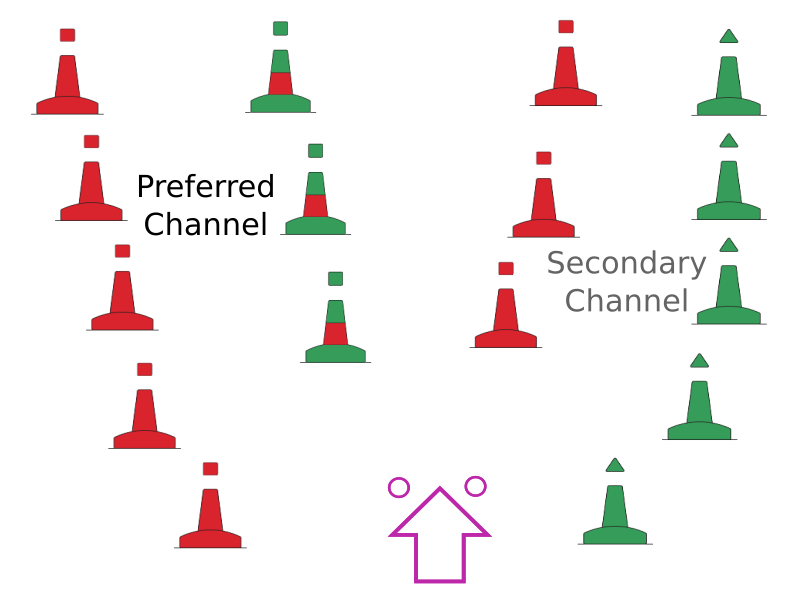
\includegraphics[width=0.9\linewidth,keepaspectratio=true]
   {resources/Channel_Port_Preferred.png}
   \captionof{figure}{Preferred channel is port so starboard marker is modified in the preferred channel}
   \vspace{20pt}
\end{center}



\newpage
\section{Special Mark}

Special marks are used to indicate specific features of interest. The nature of the special feature should be clear from the chart on which the mark appears. Special features might include:

\begin{itemize}
 \item Ocean Data Acquisition System (ODAS) bouys
 \item Traffic separation schemes
 \item Spoil grounds
 \item Military exercise zones
 \item Cables or pipelines
 \item Recreation zones
 \item Boundaries of anchorage areas
 \item Structures such as offshore renewable energy installations
 \item Aquaculture
\end{itemize}


Special marks are yellow and may carry a topmark in the form of an X. Special marks come in a wide variety of shapes as the only stipulation is that they must not conflict with shapes used for lateral water marks\footnote{If a special mark has the same shape as a lateral mark, there’s a potential for it to be misinterpreted as such under conditions of poor visibility. For this reason, a special mark on the port side must not be conical as it could be mistaken for a starboard lateral mark. Similarly, a special mark on the starboard side must not be cylindrical. A special mark on the port side may be cylindrical since that would not conflict with the lateral marks.}



\newpage
\section{Safe Water Mark}
Safe Water marks serve to indicate that there is navigable water all round the mark. These include centre line marks and mid-channel marks. Such a mark may also be used to indicate channel entrance, port or estuary approach, or landfall.

Safe water marks may be either a sphere or else a spar or pillar with a spherical topmark. They will always be coloured with red and white vertical stripes. The topmark is a solid red colour.


\begin{center}
   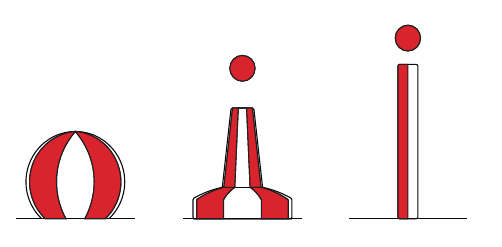
\includegraphics[width=0.9\linewidth,keepaspectratio=true]
   {resources/Safe_Water_Marks.png}
   \captionof{figure}{Safe Water Marks}
   \vspace{20pt}
\end{center}



\newpage
\section{Isolated Danger Mark}
An isolated danger mark is placed on, or near to a danger that has navigable water all around it. The isolated danger mark has a distinctive topmark consisting of two black spheres as shown below.


\begin{center}
   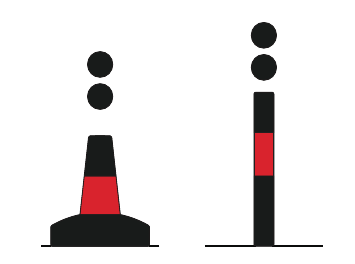
\includegraphics[width=0.9\linewidth,keepaspectratio=true]
   {resources/Isolated_Danger_Marks.png}
   \captionof{figure}{Isolated Danger Marks}
   \vspace{20pt}
\end{center}

\newpage
\section{New Danger Mark}
The term “New Danger” is used to describe newly discovered hazards not yet shown in nautical documents. ‘New Dangers’ include naturally occurring obstructions such as sandbanks or rocks as well as man-made dangers such as wrecks.

The mark may either be a pillar or a spar and may have a yellow cross topmark.


\begin{center}
   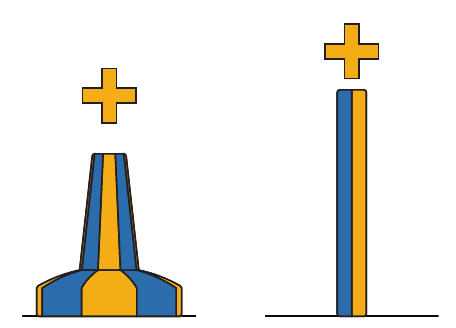
\includegraphics[width=0.9\linewidth,keepaspectratio=true]
   {resources/New_Danger_Mark.png}
   \captionof{figure}{New Danger Marks}
   \vspace{20pt}
\end{center}



\chapter{Steering and Sailing Rules}

\section{Scope of the COLREGS}
Part B of the COLREGS describes the steering and sailing rules. Regardless of the specific scenario or visibility conditions, the following two rules apply:

\begin{itemize}
 \item Every vessel shall at all times maintain a proper look-out by sight and hearing as well as by all available means appropriate in the prevailing circumstances and conditions so as to make a full appraisal of the situation and of the risk of collision.

 \item Every vessel shall at all times proceed at a safe speed so that she can take proper and effective action to avoid collision and be stopped within a distance appropriate to the prevailing circumstances and conditions.
\end{itemize}


The following are the main points covered in the steering and sailing rules


\textbf{Sailing Vessels}
When two sailing vessels are approaching, a vessel on a port tack should give way to a vessel on a starboard tack. A “port tack” means that the vessel has the wind coming from the port side.


If both vessels are on the same tack, the vessel to windward (that is, upwind), should give way to the vessel to leeward (downwind).


\textbf{Motor Vessels Head On}
When two power-driven vessels are meeting head on, each should move to starboard so that they pass port to port

\textbf{Motor Vessels Crossing}
When two power-driven vessels are crossing the vessel which has the other on their starboard side should keep out of the way

\textbf{Overtaking}
Any vessel that is overtaking should keep out of the way of the vessel being overtaken. This applies regardless of what type of vessels (motor or sail) are involved

\textbf{Responsibilities}
The full set of responsibilities are described in rule 18 of the COLREGS, part B. The main points are summarised below:

\begin{itemize}
 \item A powered vessel should keep out of the way of a sailing vessel.
 \item A sailing vessel should keep out of the way of:
 \begin{itemize}
   \item  A vessel not under command
   \item  A vessel with restricted ability to manoeuvre
   \item  A vessel engaged in fishing
 \end{itemize}
\end{itemize}


\newpage
\section{Traffic Separation Schemes}
A traffic separation scheme (TSS) is used to regulate the direction of shipping in busy areas to avoid congestion. An example TSS from the English Channel is shown below

\begin{center}
   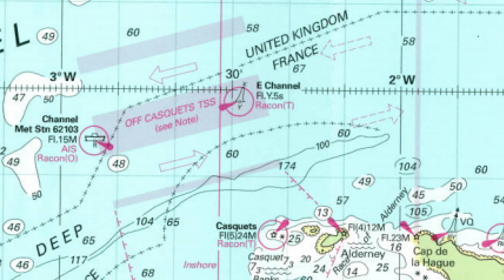
\includegraphics[width=0.9\linewidth,keepaspectratio=true]
   {resources/Traffic_Separation.png}
   \captionof{figure}{Traffic Separation Scheme}
   \vspace{20pt}
\end{center}

The direction of travel is indicated with the purple arrows and the area between these (in shaded purple) should be avoided.

It may occasionally be necessary for a vessel to cross a traffic separation zone. In this case, it’s very important that the vessel should cross the zone heading at right angles in order to minimise the time spent crossing the traffic lanes.

This latter point can cause some confusion, it’s important to remember that while the current could cause your vessel to deviate from the shortest course, you should not try to correct for this. You want to minimise the time that you spend in the traffic lanes, not the distance that you cover.

\begin{center}
   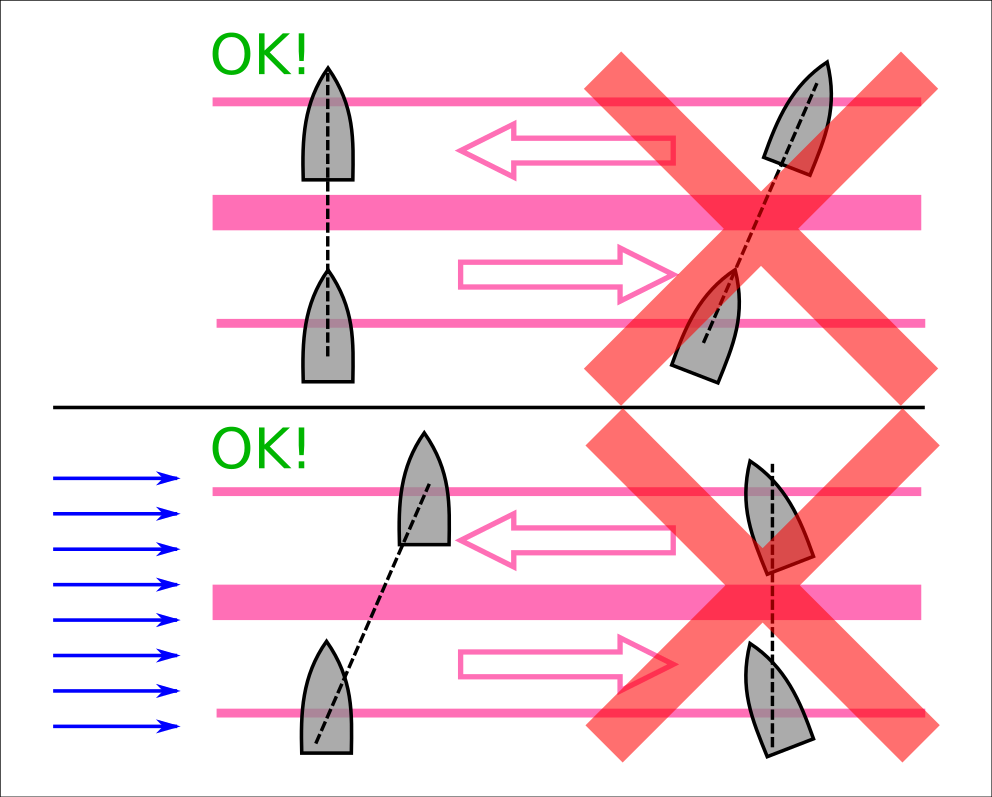
\includegraphics[width=0.9\linewidth,keepaspectratio=true]
   {resources/TSS_Crossing.png}
   \captionof{figure}{Crossing a Traffic Separation Scheme}
   \vspace{20pt}
\end{center}



\chapter{Charts and Tides}
Below is an extract from an admiralty chart covering an area around Dunstaffnage in western Scotland.


\begin{center}
   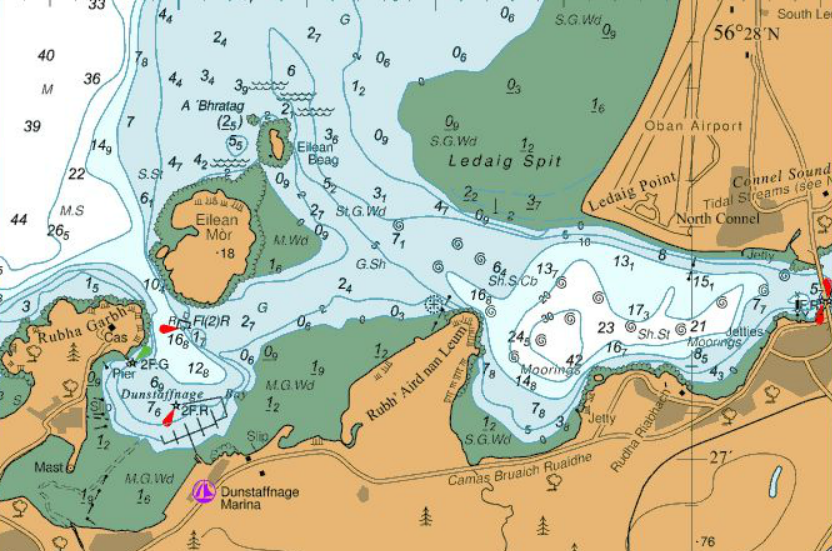
\includegraphics[width=0.9\linewidth,keepaspectratio=true]
   {resources/Chart.png}
   \captionof{figure}{Example Chart}
   \vspace{20pt}
\end{center}

The areas in shades varying between blue and white represent the sea and the depth is shown at various points. In the example below, the depth at the indicated point is 2.4 metres (the subscript value represents decimetres, that is, 1 tenth of a meter)\footnote{In this particular chart, depths are in meters but some charts (especially those published in the US) use either feet or fathoms (a fathom is 6 feet).}

\begin{center}
   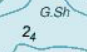
\includegraphics[width=0.2\linewidth,keepaspectratio=true]
   {resources/Depth.png}
   \captionof{figure}{Depth Indicator}
\end{center}

The actual depth at a particular time usually depends on the tide so a decision must be made as to which depth to indicate on the chart. A number of different levels might be chosen, for example, Lowest Astronomical Tide (LAT) or Mean Lower Low Water (MLLW). This level is called the chart datum and most charts (outside of the United States) use LAT as the chart datum.

Since LAT represents the lowest possible tide, the value shown indicates the minimum depth that can be expected at the marked location. Tide tables usually indicate the height above chart datum so the actual height you should expect to encounter is the value shown on the chart plus the height of the tide at the time you expect to be there.
The areas shown in green represent areas that might be above or below the waterline depending on the tide. The numbers on the green area represent the height of the area above chart datum. This value is referred to as the drying height.

In the example below, if the tide were at its lowest possible level (LAT), the green area would be 1.2 meters above the level of the sea.

\begin{center}
   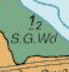
\includegraphics[width=0.15\linewidth,keepaspectratio=true]
   {resources/Drying_Height.png}
   \captionof{figure}{Drying Height}
\end{center}

Note that the numbers indicating drying height have an underline below the meters value. This is to distinguish them from depth indicators.

\begin{itemize}
  \item At a tide height of 0.5 meters, the green area would be 0.7 meters above the level of the sea.
  \item At a tide height of 1.6 meters, the green area would be below water, to a depth of 0.4 meters.
\end{itemize}

The areas shown in brown represent land, these areas are expected never to be under water.

\newpage
\section{Tidal Heights}
Apart from Lowest Astronomical Tide (LAT), there are some other key heights that are important to know about. These are summarised in the diagram below:


\begin{center}
   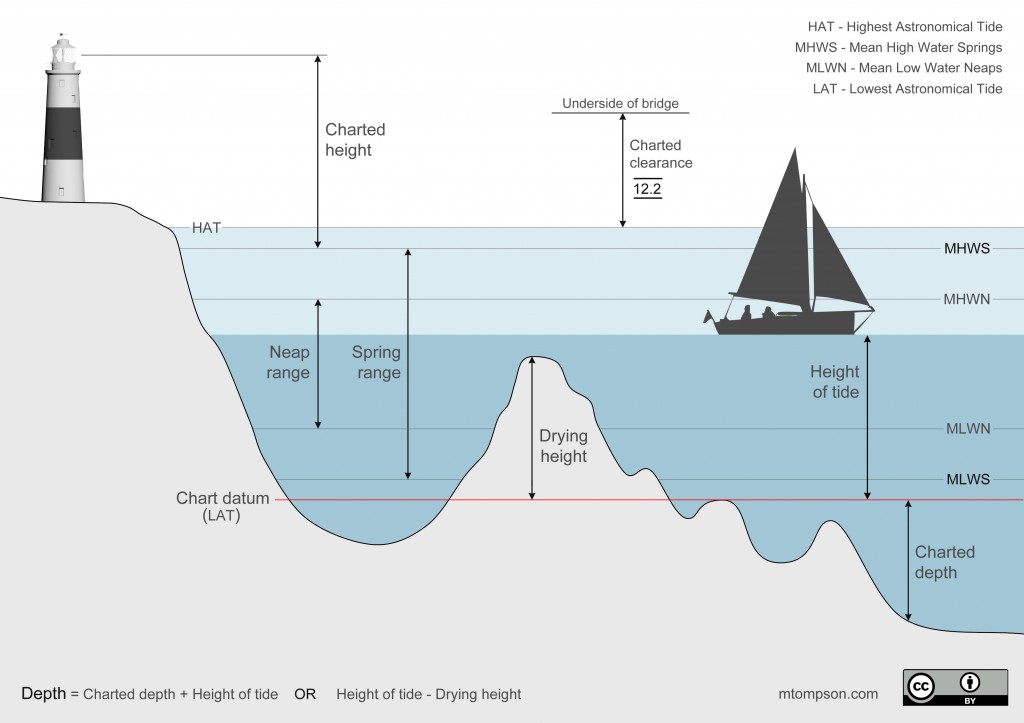
\includegraphics[width=0.9\linewidth,keepaspectratio=true]
   {resources/Tidal_Heights.jpg}
   \captionof{figure}{Tidal Heights}
   \vspace{20pt}
\end{center}

The depth at a blue or white area is the height of the tide + chart datum. For areas indicated in green, the depth is the height of the tide - the drying height.


\newpage
\section{Sample Tide Table}
The table below shows the height of the tide at North Wall in Dublin during the month of April 2018. The times are adjusted for daylight savings time and the heights shown are in meters above LAT.

\begin{center}
{
\small
\setlength{\tabcolsep}{3pt}
\begin{tabular}{ |c|c|c|c|c|c|c|c|c|c|c|c| }
 \hline
 \multicolumn{12}{|c|}{\textbf{Tide at North Wall Dublin – April 2018}} \\
\hline
& \textbf{\shortstack{\rule{0pt}{2.8ex}Time\\HH:MM}} 
& \textbf{\shortstack{\rule{0pt}{2.8ex}Height\\metres}} 
&  
& \textbf{\shortstack{\rule{0pt}{2.8ex}Time\\HH:MM}} 
& \textbf{\shortstack{\rule{0pt}{2.8ex}Height\\metres}} 
&  
& \textbf{\shortstack{\rule{0pt}{2.8ex}Time\\HH:MM}} 
& \textbf{\shortstack{\rule{0pt}{2.8ex}Height\\metres}} 
&  
& \textbf{\shortstack{\rule{0pt}{2.8ex}Time\\HH:MM}} 
& \textbf{\shortstack{\rule{0pt}{2.8ex}Height\\metres}} \\

\hline
\multirow{4}{*}{\textbf{\shortstack{01\\Sun}}} & 00:53 & 3.93 &
\multirow{4}{*}{\textbf{\shortstack{02\\Mon}}} & 01:24 & 3.90 &
\multirow{4}{*}{\textbf{\shortstack{03\\Tue}}} & 01:57 & 3.86 &
\multirow{4}{*}{\textbf{\shortstack{04\\Wed}}} & 02:33 & 3.80 \\
& 06:29 & 0.45 & & 07:06 & 0.44 & & 07:42 & 0.49 & & 08:23 & 0.59 \\
& 13:11 & 4.13 & & 13:45 & 4.07 & & 14:22 & 3.97 & & 15:03 & 3.84 \\
& 18:54 & 0.25 & & 19:30 & 0.35 & & 20:09 & 0.50 & & 20:48 & 0.70 \\

\hline
\multirow{4}{*}{\textbf{\shortstack{05\\Thu}}} & 03:13 & 3.71 &
\multirow{4}{*}{\textbf{\shortstack{06\\Fri}}} & 03:57 & 3.59 &
\multirow{4}{*}{\textbf{\shortstack{07\\Sat}}} & 04:45 & 3.43 &
\multirow{4}{*}{\textbf{\shortstack{08\\Sun\\ 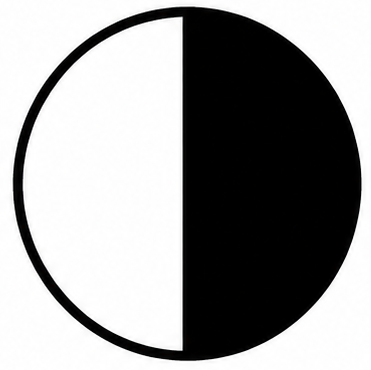
\includegraphics[height=0.35cm]{resources/moon-phases-wb.png}}}} & 05:46 & 3.27 \\
& 09:07 & 0.75 & & 09:57 & 0.93 & & 10:53 & 1.14 & & 11:55 & 1.32 \\
& 15:46 & 3.67 & & 16:35 & 3.47 & & 17:33 & 3.26 & & 18:49 & 3.11 \\
& 21:31 & 0.92 & & 22:19 & 1.16 & & 23:15 & 1.40 & & - & - \\

\hline
\multirow{4}{*}{\textbf{\shortstack{09\\Mon}}} & 00:20 & 1.58 &
\multirow{4}{*}{\textbf{\shortstack{10\\Tue}}} & 01:33 & 1.64 &
\multirow{4}{*}{\textbf{\shortstack{11\\Wed}}} & 02:49 & 1.52 &
\multirow{4}{*}{\textbf{\shortstack{12\\Thu}}} & 03:45 & 1.31 \\
& 07:08 & 3.17 & & 08:21 & 3.20 & & 09:23 & 3.33 & & 10:13 & 3.50 \\
& 13:04 & 1.41 & & 14:33 & 1.36 & & 15:24 & 1.19 & & 16:08 & 0.98 \\
& 20:03 & 3.08 & & 21:09 & 3.18 & & 22:04 & 3.34 & & 22:48 & 3.51 \\

\hline
\multirow{4}{*}{\textbf{\shortstack{13\\Fri}}} & 04:24 & 1.08 &
\multirow{4}{*}{\textbf{\shortstack{14\\Sat}}} & 04:57 & 0.85 &
\multirow{4}{*}{\textbf{\shortstack{15\\Sun}}} & 05:26 & 0.65 &
\multirow{4}{*}{\textbf{\shortstack{16\\Mon\\ 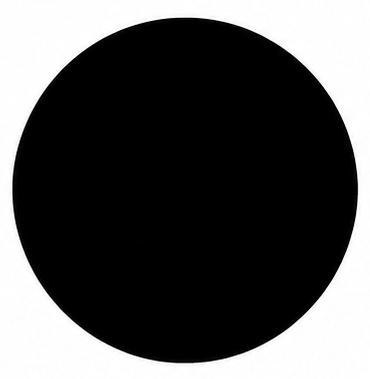
\includegraphics[height=0.35cm]{resources/moon-phases-b.png}}}} & 00:20 & 3.91 \\
& 10:54 & 3.67 & & 11:28 & 3.82 & & 12:00 & 3.95 & & 05:57 & 0.48 \\
& 16:42 & 0.77 & & 17:12 & 0.58 & & 17:42 & 0.42 & & 12:34 & 4.05 \\
& 23:23 & 3.66 & & 23:52 & 3.79 & & - & - & & 18:15 & 0.32 \\

\hline
\multirow{4}{*}{\textbf{\shortstack{17\\Tue}}} & 00:52 & 4.00 &
\multirow{4}{*}{\textbf{\shortstack{18\\Wed}}} & 01:30 & 4.04 &
\multirow{4}{*}{\textbf{\shortstack{19\\Thu}}} & 02:12 & 4.04 &
\multirow{4}{*}{\textbf{\shortstack{20\\Fri}}} & 03:00 & 3.97 \\
& 06:32 & 0.37 & & 07:11 & 0.33 & & 07:55 & 0.38 & & 08:46 & 0.50 \\
& 13:12 & 4.11 & & 13:54 & 4.11 & & 14:42 & 4.05 & & 15:33 & 3.94 \\
& 18:52 & 0.30 & & 19:33 & 0.36 & & 20:18 & 0.51 & & 21:10 & 0.72 \\

\hline
\multirow{4}{*}{\textbf{\shortstack{21\\Sat}}} & 03:51 & 3.86 &
\multirow{4}{*}{\textbf{\shortstack{22\\Sun\\  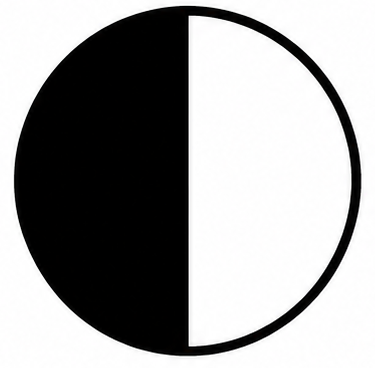
\includegraphics[height=0.35cm]{resources/moon-phases-bw.png}}}} & 04:50 & 3.72 &
\multirow{4}{*}{\textbf{\shortstack{23\\Mon}}} & 06:06 & 3.59 &
\multirow{4}{*}{\textbf{\shortstack{24\\Tue}}} & 00:33 & 1.33 \\
& 09:45 & 0.66 & & 10:52 & 0.83 & & 12:06 & 0.94 & & 07:23 & 3.55 \\
& 16:29 & 3.78 & & 17:35 & 3.61 & & 18:54 & 3.49 & & 13:24 & 0.95 \\
& 22:09 & 0.96 & & 23:16 & 1.19 & & - & - & & 20:14 & 3.49 \\

\hline
\multirow{4}{*}{\textbf{\shortstack{25\\Wed}}} & 01:54 & 1.32 &
\multirow{4}{*}{\textbf{\shortstack{26\\Thu}}} & 03:06 & 1.19 &
\multirow{4}{*}{\textbf{\shortstack{27\\Fri}}} & 04:03 & 0.99 &
\multirow{4}{*}{\textbf{\shortstack{28\\Sat}}} & 04:51 & 0.81 \\
& 08:42 & 3.63 & & 09:50 & 3.77 & & 10:48 & 3.91 & & 11:37 & 4.00 \\
& 14:37 & 0.85 & & 15:39 & 0.69 & & 16:30 & 0.54 & & 17:15 & 0.44 \\
& 21:27 & 3.58 & & 22:28 & 3.71 & & 23:18 & 3.80 & & - & - \\

\hline
\multirow{4}{*}{\textbf{\shortstack{29\\Sun}}} & 00:01 & 3.85 &
\multirow{4}{*}{\textbf{\shortstack{30\\Mon\\  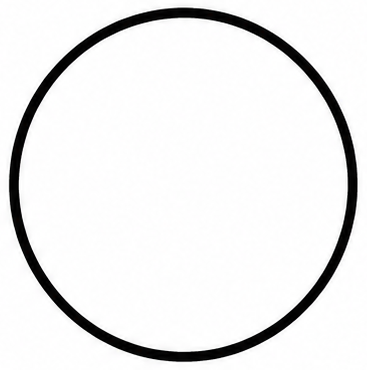
\includegraphics[height=0.35cm]{resources/moon-phases-w.png}}}} & 00:36 & 3.85 &
& & &
& & \\
& 05:33 & 0.68 & & 06:11 & 0.60 & & & & & & \\
& 12:19 & 4.02 & & 12:55 & 3.99 & & & & & & \\
& 17:56 & 0.42 & & 18:33 & 0.46 & & & & & & \\

\hline
 \multicolumn{12}{|c|}{All times given are in local time} \\
 \hline
 
\end{tabular}
}
\end{center}


\newpage
\section{Chart Symbols}


\end{document}
